\chapter{Medición de desempeño de las soluciones desarrolladas}
Se diseño un instrumento de medición (encuesta) con el fin de medir el desempeño de las automatizaciones y el porcentaje de mejora de los procesos desarrollados, esto para Automatización por medio de flujos (Power Automate). También la encuesta mide el grado de satisfacción en caso de que se haya automatizado un proceso
por medio de una aplicación (Power Apps).

\section{Diseño y validación del instrumento de medición}
Se realizó un modelo de encuesta para ser validado por los expertos donde se les preguntó su opinión con respecto a cada ítem en las tres categorías citadas: “esencial”, “útil pero no esencial” y “no necesaria”. 
\newline
El artículo \citep{tristan2008modificacion} revisa y modifica el modelo de Lawhse para calcular la razón de validez de contenido (CVR) de un instrumento, considerándolo adecuado cuando se cuenta un número pequeño de expertos y sin la necesidad de contar con consenso unánime para cada uno de los ítems. Por lo anterior, se toma el modelo \citep{tristan2008modificacion} para validar el presente instrumento. 

\begin{itemize}
	\item \textbf{CVR: }Razón de Validez de Contenido (Content Validity Ratio-CVR).
	\item \textbf{ne: }Número de expertos que tienen acuerdo en la categoría “esencial”.
	\item \textbf{N: }Número de expertos que participaron en la validación.	
\end{itemize}

\begin{equation}\label{Ecuación}
	CVR' = ne/N
\end{equation}


Este modelo establece un CVR’ por ítem mayor o igual 0.58 para ser considerado aceptable. La encuesta fue validada por tres expertos del Banco como muestra como muestra en la tabla \ref{tabla:expertos}.


\begin{table}[H]
	\centering
	\begin{tabular}{|p{4cm}|p{3cm}|p{4cm} |}
		\hline
		\multicolumn{3}{|c|}{Expertos} \\
		\hline
		\textbf{Nombre}& \textbf{Título Obtenido}&\textbf{Experiencia}\\
		\hline
		{\small Santiago Cortes Morales } & {\small Ingeniería de Sistemas.} & {\small Tech Lead Smart Digital Workspace } \\
		
		\hline
		{\small Yeison del Rio Vargas } & {\small Ingeniero de Sistemas.} & {\small 10 años de experiencia en desarrollo de proyectos TI. } \\
		
		\hline
		{\small Elvira Fernanda Paiba Castillo } & {\small Especialista en teleinformática.} & {\small 8 años de experiencia en proyectos TI. } \\
		\hline
		
		
	\end{tabular}
	\caption{Expertos}
	\label{tabla:expertos}
\end{table}

A continuación, los resultados de la validación del instrumento encuesta realizado por los expertos. En la categoría generales la pregunta 4 es aceptada para aplicar en la encuesta debido a que obtuvo un CVR mayor a 0.58. En la categoría automatización por medio de flujos todas las preguntas fueron validadas por los expertos con un CVR de 1. En la categoría de automatización por medio de flujo se suprime de la encuesta la pregunta tiene que consiguió un CVR menor a 0.58.

\begin{figure}[H]
	\centering
	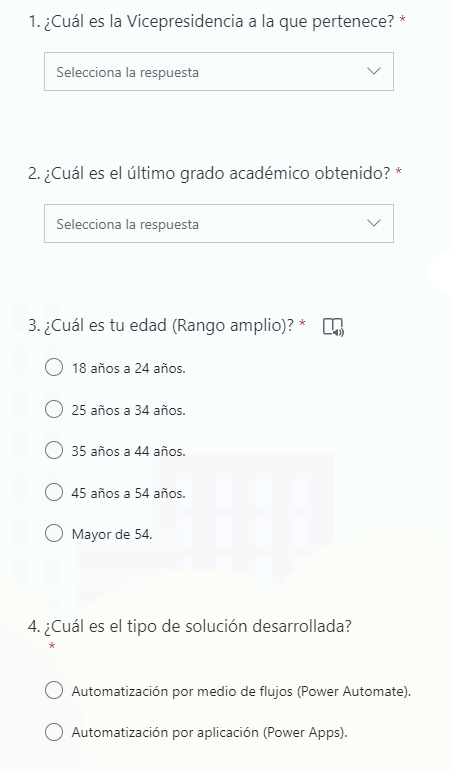
\includegraphics[scale=0.5]{Capitulo5/imagenes/f1}
	\caption{Encuesta general inicial}
	\label{fig:fomrs1}
\end{figure}


\begin{table}[H]
	\centering
	\begin{tabular}{|p{3cm}|p{3cm}|p{3cm} |}
		\hline
		\multicolumn{3}{|c|}{Generales} \\
		\hline
		\textbf{Pregunta}& \textbf{Ne}&\textbf{CVR'}\\
		\hline
		1&1&0.33\\
		\hline
		2&0&0\\
		\hline
		3&0&0\\
		\hline
		3&2&0.67\\
		\hline
			
	\end{tabular}
	\label{tabla:generales}
	\caption{Preguntas generales}
\end{table}

\begin{figure}[H]
	\centering
	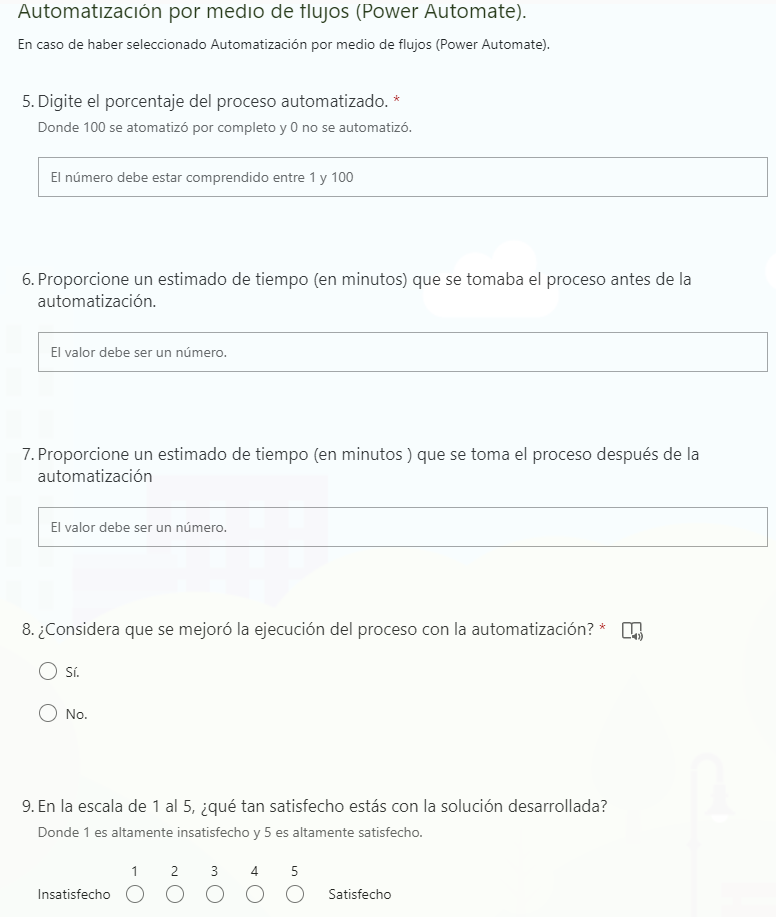
\includegraphics[scale=0.5]{Capitulo5/imagenes/fa}
	\caption{Encuesta Power Automate inicial}
	\label{fig:ea1}
\end{figure}


\begin{table}[H]
	\centering
	\begin{tabular}{|p{3cm}|p{3cm}|p{3cm} |}
		\hline
		\multicolumn{3}{|c|}{Automatización por medio de flujos (Power Automate)} \\
		\hline
		\textbf{Pregunta}& \textbf{Ne}&\textbf{CVR'}\\
		\hline
		5&3&1\\
		\hline
		6&3&1\\
		\hline
		7&3&1\\
		\hline
		8&3&1\\
		\hline
		9&3&1\\
		\hline
		
	\end{tabular}
	\label{tabla:automare}
	\caption{Preguntas power automate}
\end{table}

\begin{figure}[H]
	\centering
	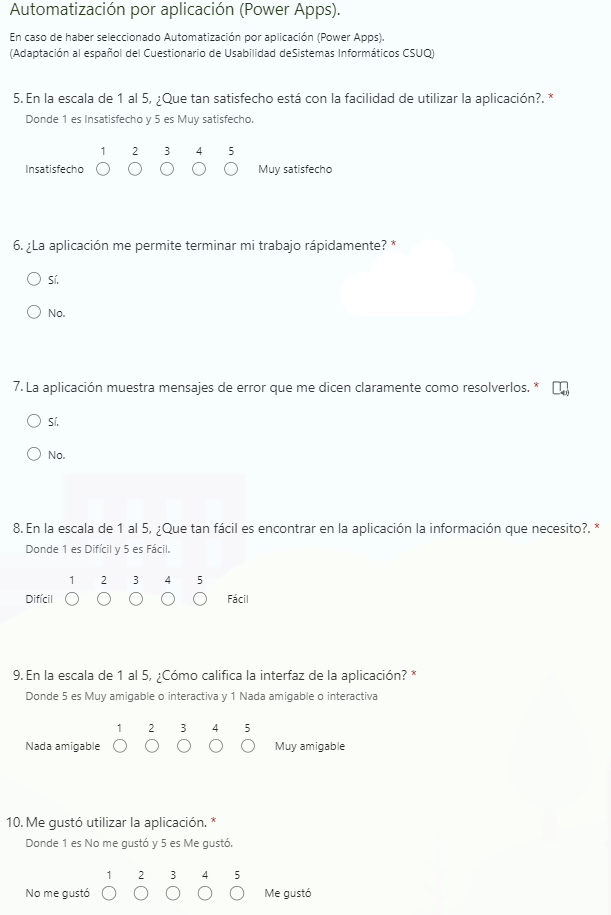
\includegraphics[scale=0.5]{Capitulo5/imagenes/fapps}
	\caption{Encuesta Power Apps inicial}
	\label{fig:eapps1}
\end{figure}


\begin{table}[H]
	\centering
	\begin{tabular}{|p{3cm}|p{3cm}|p{3cm} |}
		\hline
		\multicolumn{3}{|c|}{Automatización por medio de aplicación (Power Apps)} \\
		\hline
		\textbf{Pregunta}& \textbf{Ne}&\textbf{CVR'}\\
		\hline
		5&3&1\\
		\hline
		6&2&0.67\\
		\hline
		7&2&0.67\\
		\hline
		8&3&1\\
		\hline
		9&3&1\\
		\hline
		10&1&0.33\\
		\hline
		
	\end{tabular}
	\label{tabla:apps}
	\caption{Preguntas power apps}
\end{table}
\section{Aplicación del instrumento y análisis de resultado}


Se diseño un instrumento de medición (encuesta) con el fin de medir el desempeño de las automatizaciones y el porcentaje de mejora del proceso desarrollado, esto para Automatización por medio de flujos (Power Automate). También la encuesta mide el grado de satisfacción en caso de que se haya automatizado un proceso
por medio de una aplicación (Power Apps).



En las figuras ~\ref{fig:fomrs}, ~\ref{fig:fomrs2} y ~\ref{fig:fomrs3} se muestra la encuesta aplicada a los colaboradorres y validada por expertos.

\begin{figure}[H]
	\centering
	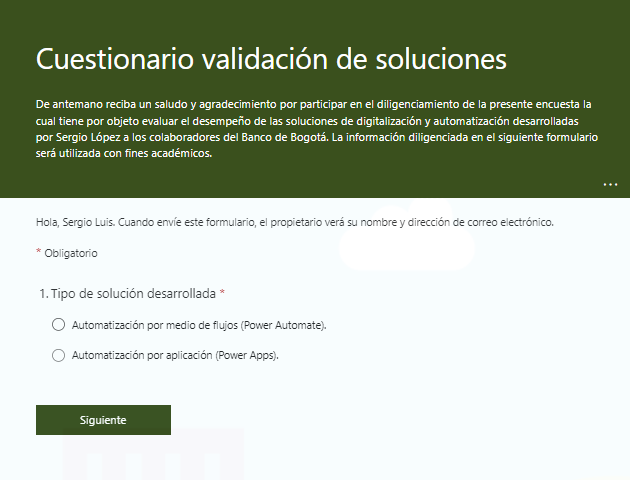
\includegraphics[scale=0.4]{Capitulo5/imagenes/1.1}
	\caption{Encuesta}
	\label{fig:fomrs}
\end{figure}
\begin{figure}[H]
	\centering
	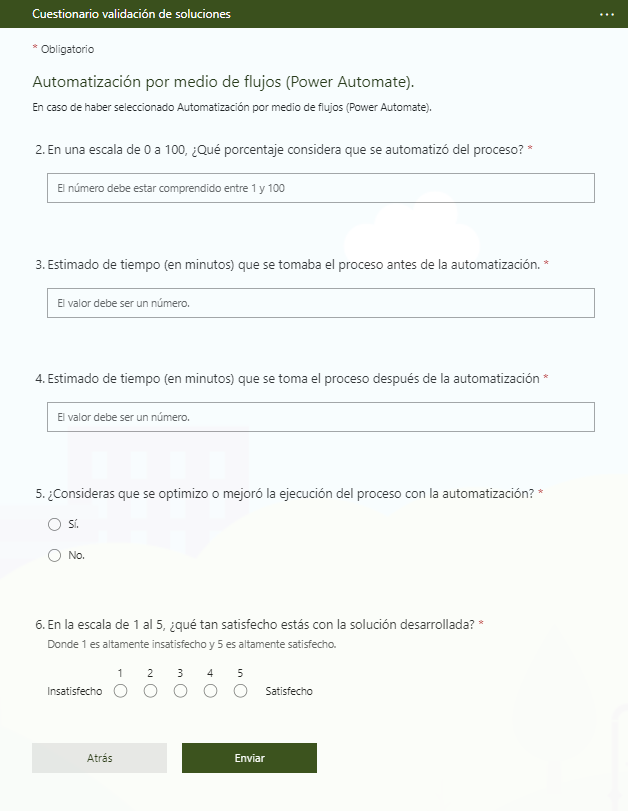
\includegraphics[scale=0.4]{Capitulo5/imagenes/a2.1}
	\caption{Encuesta (Power Automate)}
	\label{fig:fomrs2}
\end{figure}
\begin{figure}[H]
	\centering
	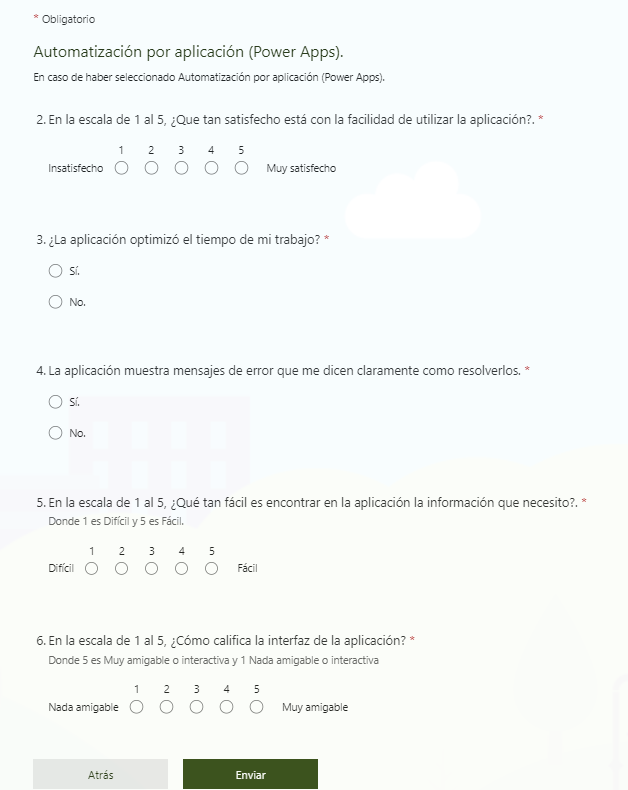
\includegraphics[scale=0.4]{Capitulo5/imagenes/app2.1}
	\caption{Encuesta (Power Apps)}
	\label{fig:fomrs3}
\end{figure}

\section{Resultado}
Los resultados de la encuesta realizados a los colaboradores dieron los resultados que nos muestran las figuras ~\ref{fig:soldes} a ~\ref{fig:inter}.

La pregunta de la figura \ref{fig:soldes} se planteó  con el fin de identificar las soluciones desarrolladas a los colaboradores.
\begin{figure}[H]
	\centering
	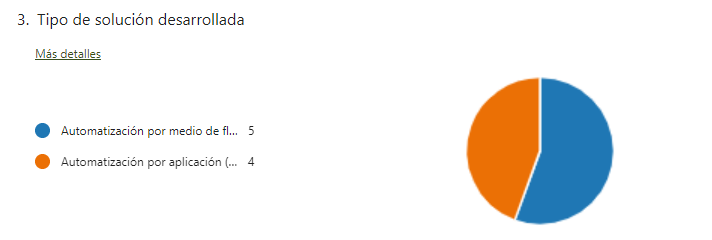
\includegraphics[scale=0.5]{Capitulo5/imagenes/4}
	\caption{Encuesta (Tipo de solución desarrollada.)}
	\label{fig:soldes}
\end{figure}

En la figura \ref{fig:porcentaje} se puede evidenciar que en un promedio del 90\% se lograron automatizar los procesos o actividades de los colaboradores del banco.

\begin{figure}[H]
	\centering
	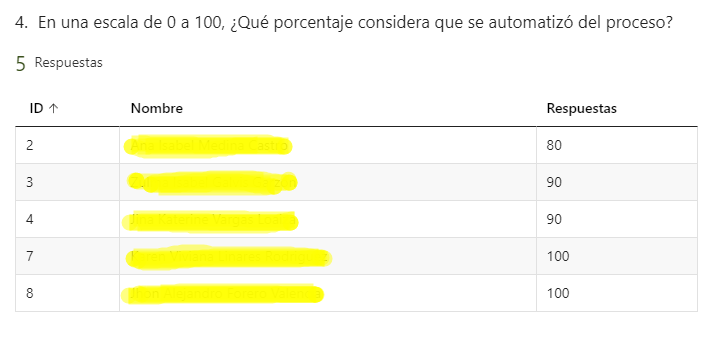
\includegraphics[scale=0.4]{Capitulo5/imagenes/5}
	\caption{En una escala de 0 a 100, ¿Qué porcentaje considera que se automatizó del proceso?}
	\label{fig:porcentaje}
\end{figure}

La pregunta de la figura \ref{fig:antes} se planteó para obtener de los colaboradores la duración de los procesos o actividades y comparar estos tiempos con el tiempo después de automatizar la actividad.

\begin{figure}[H]
	\centering
	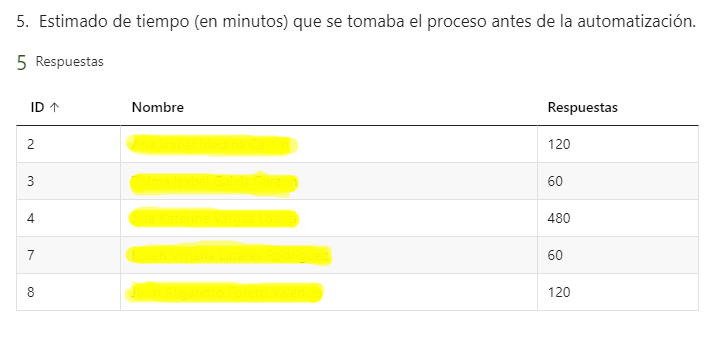
\includegraphics[scale=0.3]{Capitulo5/imagenes/6}
	\caption{Estimado de tiempo (en minutos) que se tomaba el proceso antes de la automatización.}
	\label{fig:antes}
\end{figure}

La pregunta de la figura \ref{fig:despues} se planteó para obtener de los colaboradores la duración de los procesos o actividades después de automatizado el proceso y se logró evidenciar una disminución considerable de tiempo en comparación con los las respuestas de la figura \ref{fig:antes}, dejando así en evidencia que se optimizó en cuestión de tiempo todos los proceso.


\begin{figure}[H]
	\centering
	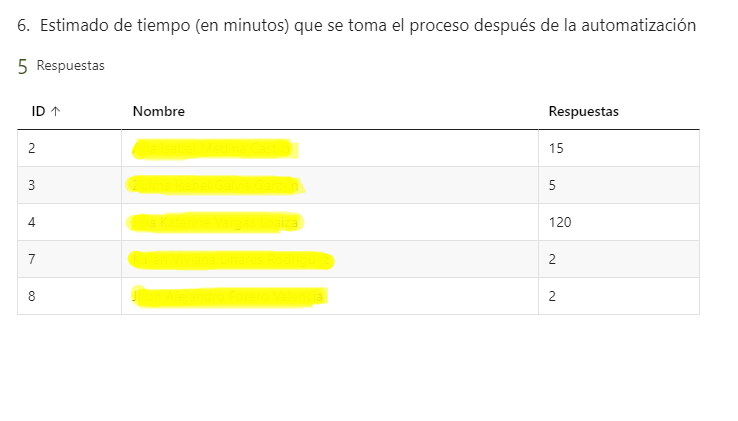
\includegraphics[scale=0.4]{Capitulo5/imagenes/7}
	\caption{Estimado de tiempo (en minutos) que se toma el proceso después de la automatización.}
	\label{fig:despues}
\end{figure}


En la figura \ref{fig:optimizo} se muestran los resultados de la pregunta \textit{¿Consideras que se optimizó o mejoró la ejecución del proceso con la automatización?} donde su logra evidenciar que en un 100\% se logró optimizar la ejecución de los procesos de los colaboradores, demostrando así que fueron desarrolladas con éxito múltiples soluciones a los colaboradores del banco.
\begin{figure}[H]
	\centering
	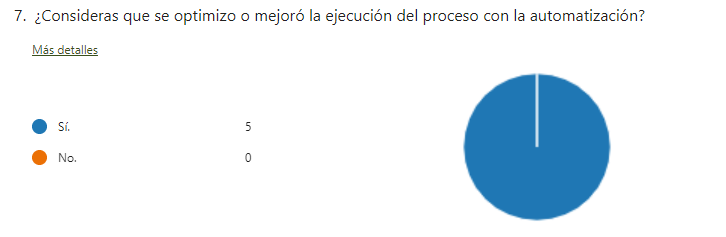
\includegraphics[scale=0.4]{Capitulo5/imagenes/8}
	\caption{¿Consideras que se optimizo o mejoró la ejecución del proceso con la automatización?}
	\label{fig:optimizo}
\end{figure}

En la figura \ref{fig:satisfecho} se logra evidenciar que el 100\% de los colaboradores a los que se les desarrolló una solución se sienten satisfechos con las soluciones desalloradas.
\begin{figure}[H]
	\centering
	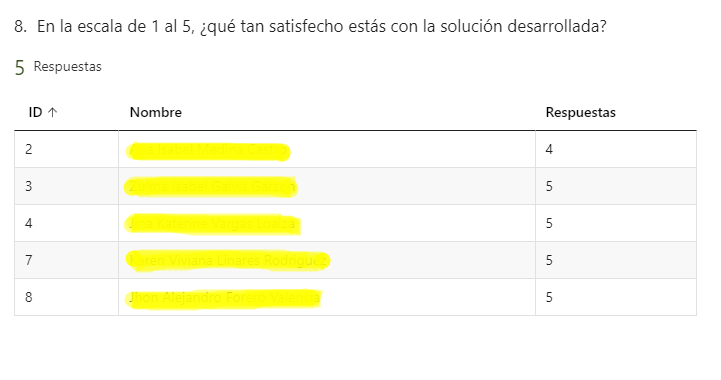
\includegraphics[scale=0.4]{Capitulo5/imagenes/9}
	\caption{Encuesta (En la escala de 1 al 5, ¿qué tan satisfecho estás con la solución desarrollada?)}
	\label{fig:satisfecho}
\end{figure}

En la figura \ref{fig:aplica} se les pregunta a los colaboradores si consideran que la aplicación diseñada es fácil de usar, un promedio del 4.86\% en una escala de 1 a 5 considera que la aplicación es fácil de usar, generando así una buena experiencia de usuario al usar la aplicación.
\begin{figure}[H]
	\centering
	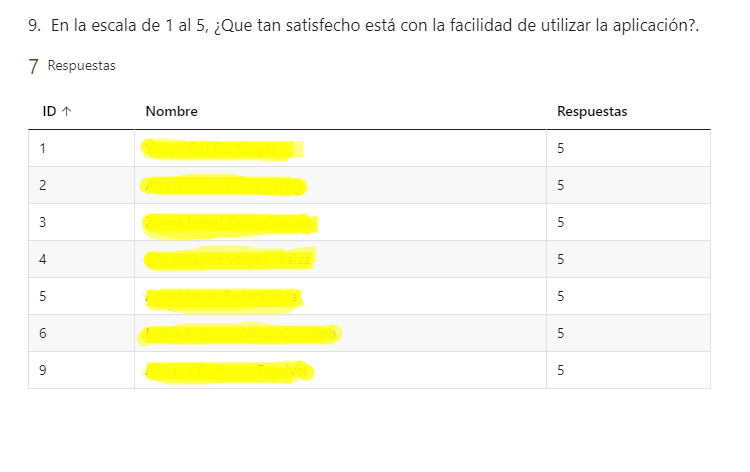
\includegraphics[scale=0.4]{Capitulo5/imagenes/10}
	\caption{Encuesta (En la escala de 1 al 5, ¿Que tan satisfecho está con la facilidad de utilizar la aplicación?.)}
	\label{fig:aplica}
\end{figure}

En la figura \ref{fig:tiempodetra} se logra evidenciar que el 100\% de los colaboradores a los que se les desarrolló una aplicación considera que la aplicación optimizó el tiempo de su trabajo, demostrando así que las aplicaciones además de brindar una buena experiencia de usuario cumple con sus funciones.

\begin{figure}[H]
	\centering
	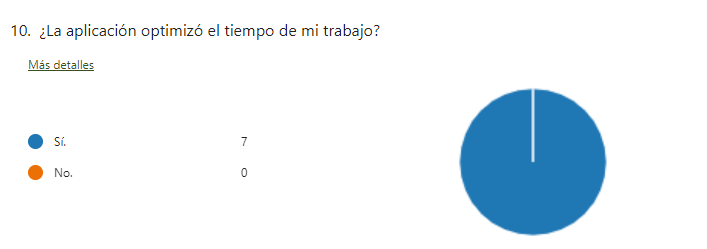
\includegraphics[scale=0.5]{Capitulo5/imagenes/11}
	\caption{¿La aplicación optimizó el tiempo de mi trabajo?}
	\label{fig:tiempodetra}
\end{figure}

La figura \ref{fig:errorsmen} nos muestra las respuestas de los colaboradores donde en un promedio de 4.77\% consideran que la aplicación cuando genera un error les muestra como deben resolverlos al mostrar los errores y como resolverlos le damos la posibilidad a los colaboradores de solventar dichos errores y continuar así con su trabajo.
\begin{figure}[H]
	\centering
	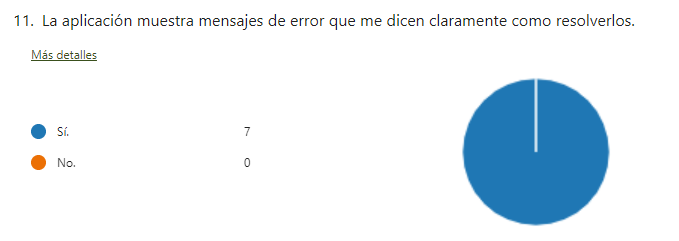
\includegraphics[scale=0.5]{Capitulo5/imagenes/12}
	\caption{La aplicación muestra mensajes de error que me dicen claramente como resolverlos.}
	\label{fig:errorsmen}
\end{figure}

En la figura \ref{fig:falic} se muestran los resultados de si es fácil o no encontrar la información que necesitan donde con un promedio de 4.88\% consideran que es fácil encontrar en la aplicación la información que necesitan.
\begin{figure}[H]
	\centering
	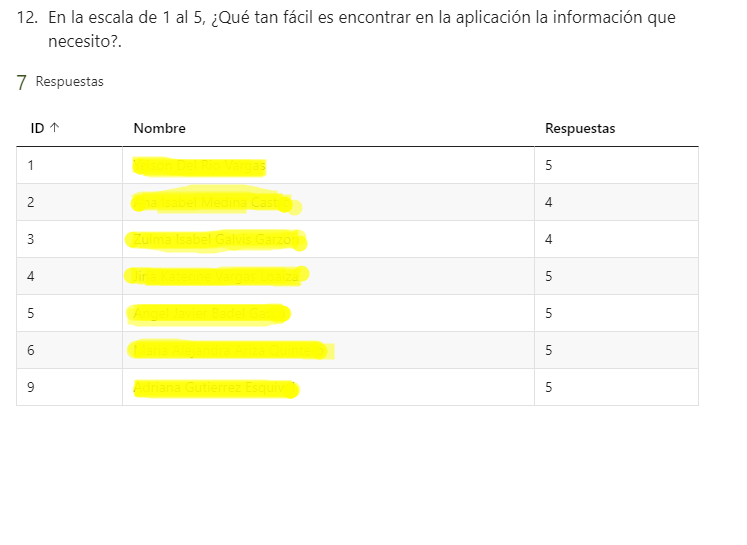
\includegraphics[scale=0.4]{Capitulo5/imagenes/13}
	\caption{En la escala de 1 al 5, ¿Qué tan fácil es encontrar en la aplicación la información que necesito?.}
	\label{fig:falic}
\end{figure}

En la figura \ref{fig:inter} 
se muestran los resultados de sí  les gusta la interfaz de la aplicación desarrollada donde con un promedio de 4.88\% les gustó la interfaz, con esto la aplicación tiene una experiencia de usuario agradable debido a que además de ser fácil de usar y la información se encuentra fácilmente también tiene una interfaz agradable, esto se concluye con los resultados obtenidos de las encuestas.
\begin{figure}[H]
	\centering
	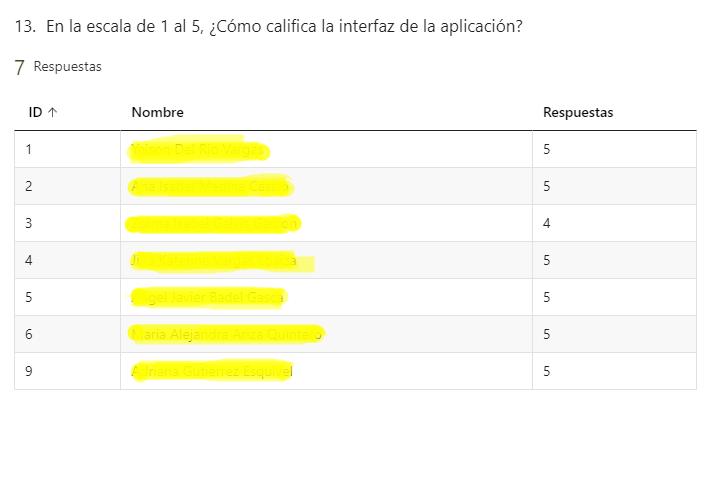
\includegraphics[scale=0.3]{Capitulo5/imagenes/14}
	\caption{En la escala de 1 al 5, ¿Cómo califica la interfaz de la aplicación?}
	\label{fig:inter}
\end{figure}



